\chapter{Architecture Overview}
\label{ch:architecture}

This serving stack is built to fail its own boot. About forty source
patches are applied to the inference engine at container start, each one
validated against pinned bytes and chained with \code{|| exit 1}. If a
single patch no longer applies cleanly, the container dies before
\code{exec vllm} ever runs --- a failed patch is a failed boot, never a
silently stock server. The engine itself is a prebuilt image that the
repository never rebuilds, pinned by manifest digest; the checkpoint is
pinned by revision. Why would anyone run a heavily modified engine this way
instead of maintaining a fork?

That question is the key to the whole design. Most serving stacks are
described by what they contain; this one is better described by what it
\emph{refuses to do}. It refuses to fork and rebuild its inference engine,
refuses to run unpinned artifacts, and refuses to boot if any of its
runtime modifications cannot be proven to apply cleanly. The result is a
layered architecture in which every layer is either pinned by cryptographic
digest or applied fail-closed at boot. This chapter walks the layers top to
bottom, follows one request through the running system, and introduces the
community lineage that produced it --- the map the remaining chapters fill
in.

For an inference engineer, the practical stakes are provenance and
rollback: when a two-node engine misbehaves, the first question is always
\emph{which bytes are actually running}. This architecture is arranged so
that the question has a checkable answer. Understanding what is pinned,
what is patched, and what fails closed is prerequisite to every debugging,
patching, and operations chapter that follows --- and it is the reason
fixes made here are portable to anyone else running the same pinned image.

\section{The layer cake}
\label{sec:architecture:layers}

\Cref{fig:architecture:stack} shows the stack. Rather than walking it as an
inventory, read it through the three refusals --- every layer exists to
enforce one of them.

\paragraph{What is pinned.} Two layers answer ``which bytes are running.''
The checkpoint, \code{deepseek-ai/DeepSeek-V4-Flash-Vision-Exp}, is pinned
to revision \code{86f746b3}\ldots{} in the HuggingFace cache, and it
supplies not only weights but executable behavior. Its
\repofile{encoding/encoding_dsv4.py} package replaces the usual Jinja chat
template: message rendering, reasoning-effort control, and DSML tool-call
parsing are all checkpoint Python that the runtime installs into vLLM at
boot (\Cref{ch:model}). Above it sits the runtime image, the prebuilt
Anemll \repofile{ghcr.io/anemll/dspark-vllm-gx10:0.1.1}, pinned by
manifest digest (\code{sha256:a8394849}\ldots) in
\repofile{.env.dspark.example} --- a vLLM fork
(\code{0.25.2.dev0+g752a3a504}) with GB10 kernels: the B12X MoE backend,
FlashInfer's SM120 sparse-MLA family, DeepGEMM, Triton, and TileLang. The
repository never rebuilds this image; it \emph{patches} it.

\paragraph{What is patched.} The patch train: about forty source patches,
mounted read-only into the container and applied by the Compose entrypoint
\emph{before} \code{exec vllm} --- the fail-closed mechanism from the
opening page, formalized and enforced in \Cref{ch:patches}. The
orchestration around the train is what keeps two machines applying it
identically. The Compose entrypoint \emph{is} the patch orchestrator; the
launcher, \repofile{start-deepseek-v4-flash-dspark.sh}, normalizes
configuration, validates the fabric, syncs patches to the worker over SSH,
runs patcher preflights on both ranks, starts worker-first, then
health-polls, smokes, and warms the JIT caches (\Cref{ch:operations}).

\paragraph{What is proven.} Configuration is one file,
\repofile{.env.dspark}, sourced through a normalizing snapshot (BOM/CRLF
stripped, atomically published to the worker with mode 0600). Every switch
is documented in a three-lane matrix --- registered on this image,
Stage-C-only no-op, or launcher-side --- in \repofile{docs/ENVS.md}
(\Cref{ch:profile}). The whole assembly is then verified twice. A CPU-only
CI gate (\repofile{scripts/ci-validate.sh}) locks wiring, defaults, and
fail-closed behavior on every push, while a live audit suite ---
throughput, speculative-decode health, long-context retrieval, tool
batteries, garble sweeps --- answers ``is this deployment actually good?''
on the real pair (\Cref{ch:measurement}).

Taken together the three refusals produce one property worth naming: at any
moment the running system reduces to a short checkable list --- a checkpoint
revision, an image digest, a set of per-patch byte hashes, and one normalized
configuration snapshot.

\begin{figure}[htbp]
\centering
\begin{tikzpicture}[node distance=3.2mm]
  \node[hbbox, text width=118mm] (verify) {\textbf{Verification} --- CPU CI gates (wiring, defaults) + live audit suite (tok/s, RULER, tools, garble)};
  \node[hbbox, text width=118mm, below=of verify] (ops) {\textbf{Orchestration} --- launcher (fabric validation, worker sync, preflights, worker-first boot, warmup) + ops scripts};
  \node[hbnode, text width=118mm, below=of ops] (cfg) {\textbf{Configuration} --- \detokenize{.env.dspark} snapshot $\rightarrow$ Compose interpolation $\rightarrow$ container env};
  \node[hbpatch, text width=118mm, below=of cfg] (patch) {\textbf{Patch train} --- $\sim$40 fail-closed, source-locked boot-time patches (\detokenize{|| exit 1})};
  \node[hbgpu, text width=118mm, below=of patch] (image) {\textbf{Runtime image} --- Anemll dspark-vllm-gx10:0.1.1, digest-pinned (vLLM fork + GB10 kernels)};
  \node[hbnode, text width=118mm, below=of image] (ckpt) {\textbf{Checkpoint} --- DeepSeek-V4-Flash-Vision-Exp @ pinned revision (weights + encoding\_dsv4.py)};
  \node[hbhost, text width=118mm, below=of ckpt] (hw) {\textbf{Hardware} --- 2$\times$ DGX Spark (GB10, 128 GB unified) + 200 Gb RoCE};
  \draw[hbarrow] (verify.south) -- (ops.north);
  \draw[hbarrow] (ops.south) -- (cfg.north);
  \draw[hbarrow] (cfg.south) -- (patch.north);
  \draw[hbarrow] (patch.south) -- (image.north);
  \draw[hbarrow] (image.south) -- (ckpt.north);
  \draw[hbarrow] (ckpt.south) -- (hw.north);
\end{tikzpicture}
\caption{The layer cake. Every layer is pinned (digest, revision, byte hash)
or applied fail-closed at boot; nothing is rebuilt, and nothing unproven is
allowed to serve. None of this is small machinery: the Compose file runs
463 lines and the launcher 1{,}753.}
\label{fig:architecture:stack}
\end{figure}

\begin{hblesson}
The central architectural bet: \emph{pin a prebuilt image and patch it at
boot} rather than maintaining a fork.
\end{hblesson}

That bet is the answer to the opening question. The pin gives byte-exact
provenance and trivially reproducible bug reports. Boot-time patching keeps
every local change a small, reviewable, individually revertable diff, and
container recreation is a guaranteed rollback to pristine upstream bytes
--- together, three properties a privately maintained fork surrenders.
\Cref{ch:patches} examines what this discipline costs and how it is
enforced, and \Cref{fig:architecture:bet} sets the two options side by side.

\begin{figure}[htbp]
\centering
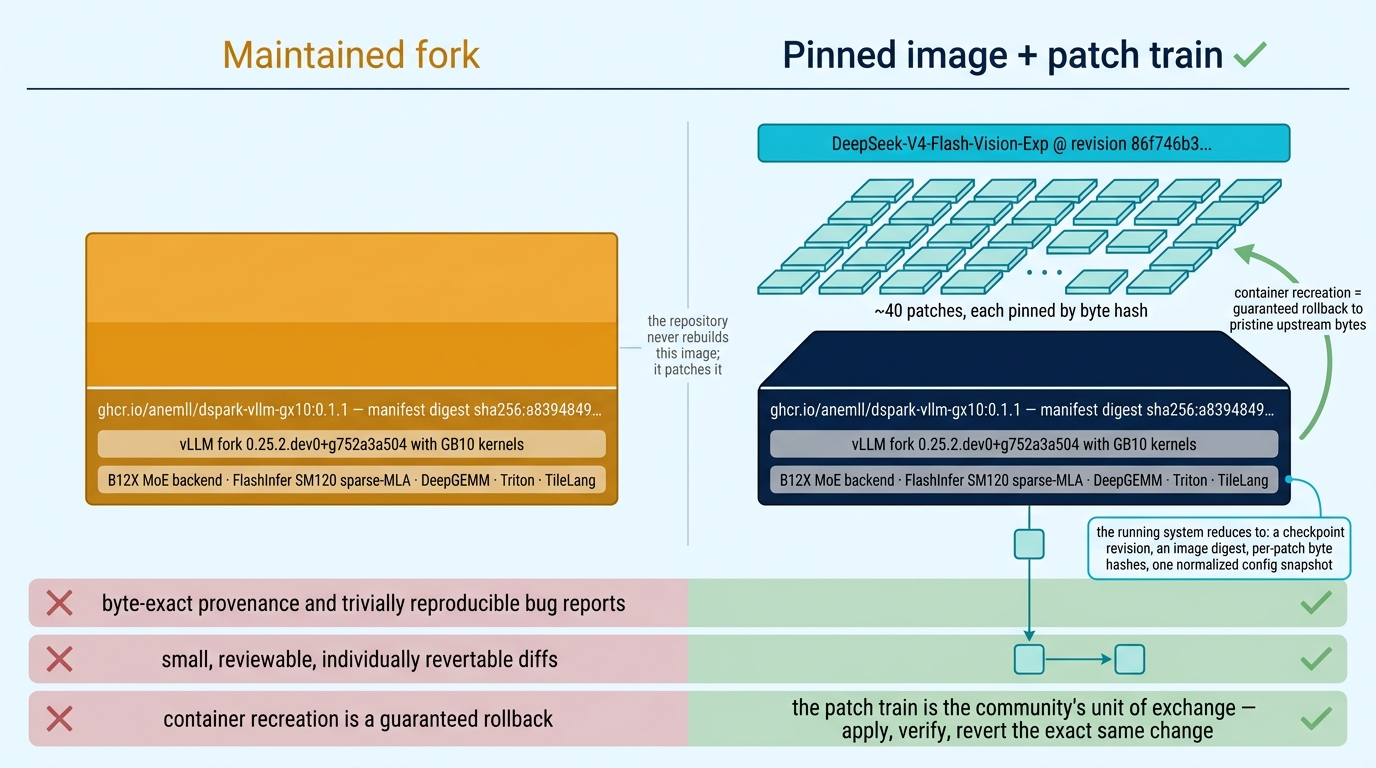
\includegraphics[width=\textwidth]{figures/ch02-central-bet.png}
\caption{The architectural bet. A maintained fork fuses local changes into
rebuilt bytes; pinning a prebuilt image and applying the patch train at boot
keeps every modification a separable, hash-pinned diff on top of bytes anyone
else can obtain. The three properties on the right are exactly what a private
fork surrenders --- and they are what makes a fix here portable to another
operator of the same image.}
\label{fig:architecture:bet}
\end{figure}

\section{The life of a request}
\label{sec:architecture:request}

The path below repays two readings: one for the sequence, one for how many
of its steps are behavior this repository added rather than inherited. To
see the layers in motion, follow one chat completion through the running
system (\Cref{fig:architecture:request}):

\begin{enumerate}
  \item A client POSTs an OpenAI-style request to
    \code{http://head:8888/v1/chat/completions} --- messages, optional
    images, tools, sampling parameters, and per-request
    \code{chat_template_kwargs} controlling thinking effort.
  \item vLLM's API layer validates it. Several of this system's patches
    live here: image parts are rejected outside \code{user} turns, truncated
    tool calls will later be re-labeled, and (opt-in) named-tool responses
    are contract-checked before returning.
  \item The \emph{checkpoint's own encoder} --- installed at boot as
    \repofile{vllm/tokenizers/deepseek_v4_encoding.py} --- renders messages
    into token IDs: role headers, \code{<think>} markers, DSML tool-result
    encoding, image placeholder tokens.
  \item The scheduler admits the request into continuous batching. Long
    prompts are \emph{chunk-prefilled} 1{,}024 tokens at a time, with an
    admission cap on concurrent partial prefills so decoding requests are
    never starved --- the hardest-won scheduler behavior in the repository
    (\ghissue{27}, \ghissue{43}; \Cref{ch:bugs}).
  \item Each engine step runs on both ranks: the head broadcasts the step
    plan to the worker over ZeroMQ; each rank streams its weight shard,
    computes, and synchronizes through $\sim$108 NCCL collectives per decode
    step over the RoCE link.
  \item The DSpark drafter proposes a block of six tokens; the target model
    verifies them in one pass; accepted tokens (typically 3--4) are appended.
    Prefix caching stores computed KV so a follow-up turn reuses the
    conversation's prefix (\Cref{ch:specdecode}).
  \item The detokenizer streams text out --- with client \code{stop} strings
    held dormant inside \code{<think>} (a patch) --- and the reasoning and
    tool-call parsers split the stream into \code{reasoning}, \code{content},
    and structured \code{tool_calls} for the response.
\end{enumerate}

\begin{figure}[htbp]
\centering
\adjustbox{max width=\textwidth}{%
\begin{tikzpicture}[node distance=4mm and 7mm]
  \node[hbnode] (cli) {client};
  \node[hbbox, right=of cli] (api) {API layer\\\scriptsize validation,\\\scriptsize contracts};
  \node[hbbox, right=of api] (enc) {encoder\\\scriptsize encoding\_dsv4\\\scriptsize $\rightarrow$ token IDs};
  \node[hbbox, right=of enc] (sched) {scheduler\\\scriptsize chunked prefill,\\\scriptsize admission caps};
  \node[hbgpu, right=of sched] (eng) {TP=2 engine\\\scriptsize rank 0 + rank 1\\\scriptsize NCCL over RoCE};
  \node[hbbox, below=of eng] (spec) {DSpark\\\scriptsize draft 6, verify 1 pass};
  \node[hbbox, left=of spec] (detok) {detokenizer\\\scriptsize stop guard};
  \node[hbbox, left=of detok] (parse) {parsers\\\scriptsize reasoning / tools};
  \node[hbnode, left=of parse] (resp) {response\\\scriptsize SSE stream};
  \draw[hbflow] (cli) -- (api);
  \draw[hbflow] (api) -- (enc);
  \draw[hbflow] (enc) -- (sched);
  \draw[hbflow] (sched) -- (eng);
  \draw[hbflow] (eng) -- (spec);
  \draw[hbflow] (spec) -- (detok);
  \draw[hbflow] (detok) -- (parse);
  \draw[hbflow] (parse) -- (resp);
  \draw[hbarrow, dashed] (spec.east) to[out=0,in=-20] node[hblabel, right]{accepted tokens} (eng.east);
\end{tikzpicture}%
}
\caption{The life of a request. Patched behavior (validation contracts, the
checkpoint encoder, admission caps, the stop-string guard) sits at almost
every stage.}
\label{fig:architecture:request}
\end{figure}

\section{Head and worker: one engine, two roles}
\label{sec:architecture:roles}

The request walkthrough treated the two ranks as interchangeable halves of
one engine; keeping them that way is a design goal in its own right. The
two containers run the \emph{same} image, the same entrypoint, and the
same patch train --- divergence between ranks is itself a failure mode the
launcher works to prevent. They differ only in role variables:
\envvar{NODE_RANK=0} on the head, which binds the HTTP server; and
\envvar{NODE_RANK=1} with \envvar{HEADLESS=1} on the worker, whose
healthcheck short-circuits to success because there is no port to probe.
The launcher enforces \emph{worker-first} startup: rank~1 must be waiting
before rank~0 initializes its TCPStore. The converse holds too --- stopping
is always pairwise, because a surviving lone rank is stale, not healthy
(\Cref{ch:operations}). \Cref{fig:architecture:boot} walks the ordering and
the hazard beside it.

\begin{hbwarning}
Docker's \code{restart: unless-stopped} policy can resurrect the two ranks
\emph{independently} after host reboots --- a split-brain hazard where one
rank is fresh and the other stale. The launcher detects an already-running
head and exits with code 3 (``already up, not an error''), and the
documentation is explicit that exit 3 is \emph{not} a health claim.
Supervised deployments set \envvar{DSPARK_RESTART_POLICY=no} and let the
unit own the lifecycle.
\end{hbwarning}

\begin{figure}[htbp]
\centering
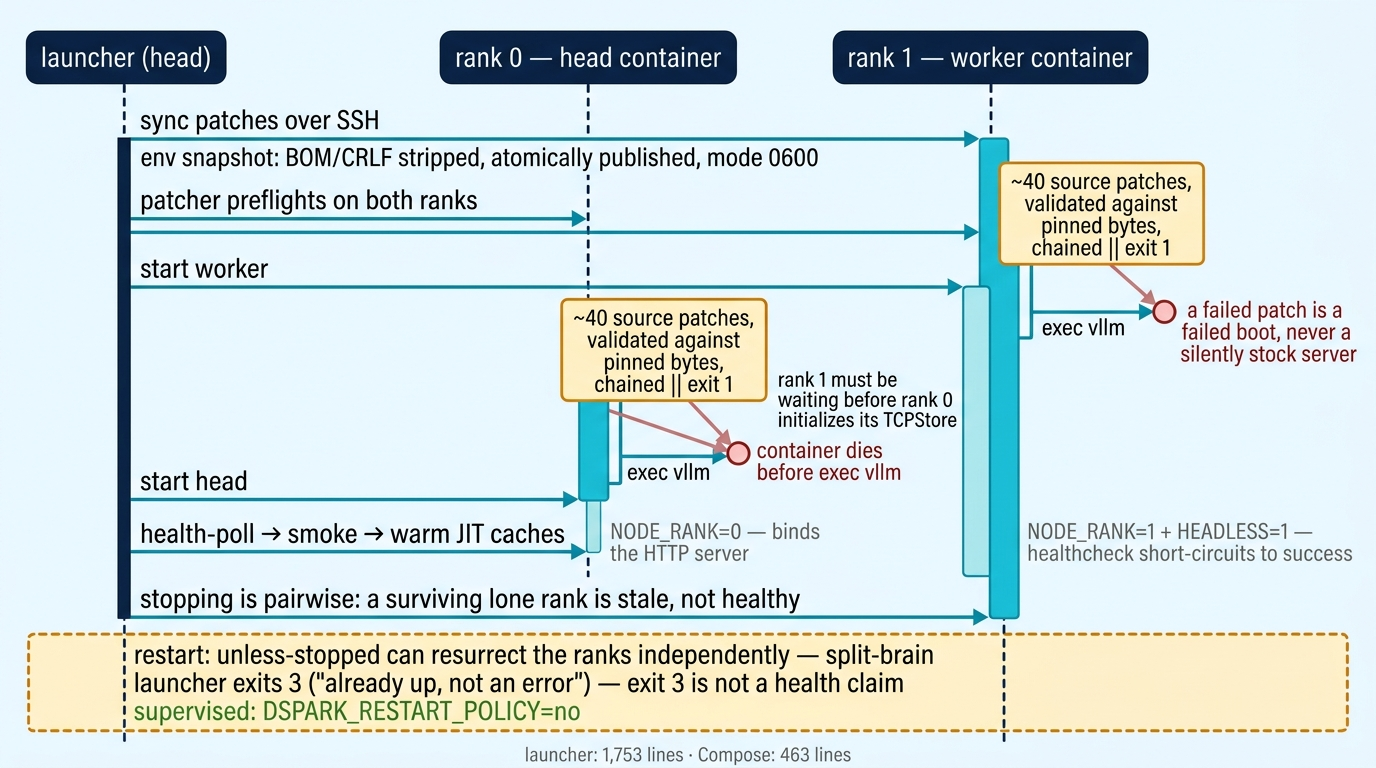
\includegraphics[width=\textwidth]{figures/ch02-boot-gate.png}
\caption{Boot, in order. The launcher normalizes configuration, validates the
fabric, syncs patches over SSH and preflights both ranks, then starts the
worker first so rank~1 is waiting before rank~0 initializes its TCPStore.
Inside each container the patch train runs before \code{exec vllm} and any
failure kills the container rather than serving stock bytes; the hazard lane
shows the converse, an unsupervised restart policy resurrecting the two ranks
independently.}
\label{fig:architecture:boot}
\end{figure}

\section{Provenance and lineage}
\label{sec:architecture:lineage}

Fail-closed patching earns its keep at boot; the pinning half of the bet
pays off somewhere less obvious. Because the runtime is a \emph{pinned
communal image} rather than a private fork, every fix in \Cref{ch:bugs} exists as a portable patch against known
bytes --- other operators of the same image can apply, verify, and revert
the exact same change. The patch train is not just a deployment mechanism;
it is the community's unit of exchange. And the community is real: this
system is the fourth generation of a lineage recorded in
\repofile{docs/SETUP.md} and \repofile{CREDITS.md}. The chain that follows
is operational information rather than courtesy: each generation owns a
distinct layer of what runs today, so placing a behavior in the lineage
narrows where its patches and its documentation live.

The chain runs from \textbf{Rafael Caricio}, who built the original
DSpark--vLLM integration and the control replica (single-stream,
unpatched), through \textbf{tonyd2wild}, who packaged the reproducible
two-node recipe --- self-contained Compose, a direct \code{vllm serve} launch,
and the worker-first start script from Mia's AI Lab --- that this repository descends
from. \textbf{drowzeys (``Keys'')} wrote the
concurrency patches that made batched DSpark \emph{correct} ---
request-stable KV slots and the ragged context path (\Cref{ch:specdecode})
--- plus the abliterated checkpoint variants.

\textbf{Anemll} ships the prebuilt GB10 image that became the pinned
runtime, replacing an earlier locally built ``Stage-C'' overlay stack that
survives as an optional lane (\Cref{ch:scaling}).
\textbf{localaiguyy} contributed the attention-group padding that unlocks a
third node (TP=3). \textbf{Mia's AI Lab} operates the cluster and maintains
the repository --- including the issue tracker whose numbered incidents
(\ghissue{21} through \ghissue{211}) structure \Cref{ch:bugs}.

\section{A map of this book}
\label{sec:architecture:map}

The remaining chapters follow the layers. \Cref{ch:model} descends into the
model itself; \Cref{ch:profile} reads the serving configuration flag by
flag; \Cref{ch:fabric} covers the network layer beneath TP.
\Cref{ch:patches} formalizes the patch discipline and \Cref{ch:bugs}
chronicles the bugs it exists to fix. \Cref{ch:specdecode} treats
speculative decoding in production depth, \Cref{ch:perf} builds the
performance model and recounts the tuning campaigns, and
\Cref{ch:measurement} documents the benchmarking doctrine that keeps the
numbers honest. \Cref{ch:operations} is the runbook; \Cref{ch:scaling}
surveys the paths beyond two nodes; \Cref{ch:lessons} distills what
transfers to any inference deployment.

\FloatBarrier
The stack is no longer software that was installed; it is a short list of
pins plus a diff applied at boot. Ask which bytes are serving and the answer
is enumerable --- one checkpoint revision, one image digest, a set of
per-patch byte hashes, one normalized configuration snapshot --- and
anything that cannot be proven against that list kills the container instead
of quietly serving stock behavior. The patch train from the opening page is
not debt owed to a fork nobody wrote; its diffs are the unit in which this
system is modified, exchanged with other operators, and rolled back.

\section*{Takeaways}

\begin{itemize}
  \item The architecture is defined by pins: checkpoint revision, image
    manifest digest, and per-patch byte hashes --- plus fail-closed
    boot-time patching instead of a forked rebuild.
  \item That bet buys three properties a private fork surrenders:
    byte-exact provenance and reproducible bug reports, local changes that
    stay small and individually revertable, and rollback by container
    recreation to pristine upstream bytes --- which is also what makes a
    fix here portable to anyone running the same pinned image.
  \item A request crosses patched behavior at nearly every stage: API
    contracts, the checkpoint's own encoder, scheduler admission caps, the
    draft/verify loop, and the stop-string-aware detokenizer.
  \item Divergence is failure: head and worker run identical bytes with
    different role variables, boot worker-first, and stop pairwise ---
    and exit 3 (``already up'') is explicitly not a health claim.
\end{itemize}

\chaptertransition{Pins and patches settle \emph{which} bytes are running;
they say nothing about what those bytes do once a request arrives. Much of
the patch train exists because some property of this particular checkpoint
--- a KV cache that tensor parallelism cannot shard, an FFN that routes on
raw token ids, a drafter whose state lives outside the engine's cache ---
made stock behavior wrong, so the train cannot be read, extended,
or safely reverted by anyone who does not know the model's anatomy. The next
chapter opens it, beginning with a configured KV dtype whose name is the
only thing separating it from another: identical bytes, different dispatch,
and one string comparison that quietly cost long-context decode a factor of
sixteen.}
